\chapter{The \texorpdfstring{\(SU(5)\)}{SU(5)} Multiplets, Leptoquark Gauge Bosons, and Proton Decay}

\lectureoverview{Grand unification becomes concrete when the Standard Model group is embedded in \(SU(5)\). To see what that statement means, we first build the necessary representation theory: the defining representation \(N\), its conjugate \(\overline N\), tensor products, symmetric and antisymmetric tensors, and the adjoint. One Standard Model family then falls into the unexpectedly economical combination \(\overline{\mathbf 5}\oplus\mathbf{10}\). The same symmetry that makes this arrangement beautiful also requires colored gauge bosons that convert quarks into leptons. Their exchange permits proton decay, forcing the unification scale toward \(10^{15}\)--\(10^{16}\,\mathrm{GeV}\). The running gauge couplings point toward a similar scale, and supersymmetry returns at the end because it makes their numerical meeting substantially sharper.}

\section{Why Begin with Group Representations?}

There are many proposed grand unified theories. Rather than survey them, we shall take apart one example and ask three questions: what makes it work, what new particles it requires, and where experiment puts it in danger. The group is \(SU(5)\), and its defining structural feature is the embedding
\begin{equation}
SU(3)_c\times SU(2)_L\times U(1)_Y
\subset SU(5).
\label{eq:l10-sm-embedding}
\end{equation}
Here \(SU(3)_c\) acts on color, \(SU(2)_L\) on weak isospin, and \(U(1)_Y\) on hypercharge.

Supersymmetry is not a premise of this construction. Neither supersymmetry nor grand unification logically implies the other. Their connection in this lecture is numerical: when the superpartner spectrum is included in the renormalization-group calculation, the three gauge couplings approach a common value more accurately.

Particles that a symmetry mixes among themselves form a representation of the symmetry group. Classifying unified particle multiplets therefore requires a little representation theory first.

\subsection{The Familiar \texorpdfstring{\(SU(2)\)}{SU(2)} Example}

The \(SU(2)\) associated with ordinary angular momentum is closely related to rotations of three-dimensional space. More precisely, \(SU(2)\) is the double cover of \(SO(3)\). Its irreducible representations are labeled by
\begin{equation}
j=0,\frac12,1,\frac32,\ldots,
\qquad
\dim(j)=2j+1.
\label{eq:l10-su2-spins}
\end{equation}
Thus a scalar is a singlet, a spin-\(\tfrac12\) particle is a doublet, and a spin-one particle is a triplet. The weak group \(SU(2)_L\) is a different physical symmetry, although its abstract group theory is the same.

\section{The Defining Representation and Its Conjugate}

For \(SU(N)\), the defining representation is the space of complex \(N\)-component columns,
\begin{equation}
\psi=
\begin{pmatrix}
\psi_1\\
\psi_2\\
\vdots\\
\psi_N
\end{pmatrix},
\qquad
\psi'_i=U_i{}^j\psi_j,
\qquad
U\in SU(N).
\label{eq:l10-defining}
\end{equation}
It is called either the defining representation or simply \(\mathbf N\). The matrices \(U\) are \(N\times N\), and the vector space on which they act has dimension \(N\).

Complex conjugation gives another \(N\)-dimensional representation,
\begin{equation}
\psi_i^*\longmapsto U_i{}^{j*}\psi_j^*,
\label{eq:l10-conjugate}
\end{equation}
denoted \(\overline{\mathbf N}\). For \(N>2\), the defining and conjugate representations are inequivalent. One may exchange which is called the particle representation and which the antiparticle representation, but after choosing a convention one must keep it fixed.

\begin{classroomqa}
\audiencequestion{Does the \(N\) in \(SU(N)\) depend on whether \(N\) is even or odd, and does it refer to the matrices? \lecturetimestamp{00:07:33}}
\lecturerresponse{There is no even--odd restriction here. \(N\) is the size of the defining matrices and also the dimension of their defining representation. Both \(\mathbf N\) and \(\overline{\mathbf N}\) have that dimension.}
\end{classroomqa}

The antiparticle of an antiparticle is the original particle. This is why interchanging the names \(\mathbf N\) and \(\overline{\mathbf N}\) changes convention rather than physics.

\section{Tensor Products and Irreducibility}

Suppose one object can occupy \(N\) internal states and another object can independently occupy the same number. Ignoring position, momentum, spin, and every quantum number except this \(SU(N)\) label, the pair has
\begin{equation}
N\times N=N^2
\label{eq:l10-product-count}
\end{equation}
states. If the first object is in state \(\psi_i\) and the second in state \(\phi_j\), their product may be written
\begin{equation}
\Psi_{ij}=\psi_i\phi_j,
\qquad
\Psi'_{ij}=U_i{}^kU_j{}^\ell\Psi_{k\ell}.
\label{eq:l10-tensor-transform}
\end{equation}
This is the tensor product \(\mathbf N\otimes\mathbf N\).

\begin{classroomqa}
\audiencequestion{Why is the answer \(N^2\), rather than \(N^2-1\), and does allowing both particles the same internal label violate the exclusion principle? \lecturetimestamp{00:10:22}}
\lecturerresponse{The two slots are distinguishable here: one object is fixed at one location and the other at another. The Pauli principle constrains the complete quantum state, including position. It does not remove any of these \(N^2\) internal-label combinations. The number \(N^2-1\) will arise later from a tracelessness condition in a different product.}
\end{classroomqa}

The \(N^2\)-dimensional product representation is generally reducible. A representation is reducible when it contains a proper subspace that the group maps into itself. The invariant subspaces can be separated and treated as smaller representations; if no such proper subspace exists, the representation is irreducible.

\subsection{Symmetric and Antisymmetric Tensors}

Every two-index tensor splits uniquely into
\begin{align}
\Psi_{ij}
&=\Psi^{(S)}_{ij}+\Psi^{(A)}_{ij},\\
\Psi^{(S)}_{ij}
&=\frac12(\Psi_{ij}+\Psi_{ji}),\\
\Psi^{(A)}_{ij}
&=\frac12(\Psi_{ij}-\Psi_{ji}).
\label{eq:l10-sym-anti}
\end{align}
The two pieces obey
\begin{equation}
\Psi^{(S)}_{ij}=\Psi^{(S)}_{ji},
\qquad
\Psi^{(A)}_{ij}=-\Psi^{(A)}_{ji}.
\end{equation}
Equation~\eqref{eq:l10-tensor-transform} preserves each condition, so group transformations never mix the symmetric and antisymmetric sectors.

\editorialnote{The lecture leaves the general counting as an exercise. The symmetric and antisymmetric dimensions are \(N(N+1)/2\) and \(N(N-1)/2\), respectively, and their sum is \(N^2\).}

\begin{figure}[htbp]
\centering

\includegraphics[width=0.78\textwidth]{lecture_10_figure_02.png}
\lectureframe{00:17:57.500}
\caption{The completed board decomposition for two spin-\(\tfrac12\) states: three symmetric states and one antisymmetric state.}
\label{fig:l10-spin-decomposition}
\end{figure}

For the defining doublet of \(SU(2)\),
\begin{equation}
\mathbf2\otimes\mathbf2=\mathbf3_S\oplus\mathbf1_A.
\label{eq:l10-two-two}
\end{equation}
Writing the two basis states as \(u\) and \(d\), the symmetric triplet is
\begin{align}
\ket{1,1}&=\ket{uu},\\
\ket{1,0}&=\frac{1}{\sqrt2}\bigl(\ket{ud}+\ket{du}\bigr),\\
\ket{1,-1}&=\ket{dd},
\end{align}
while the antisymmetric singlet is
\begin{equation}
\ket{0,0}
=\frac{1}{\sqrt2}\bigl(\ket{ud}-\ket{du}\bigr).
\end{equation}
This is the familiar addition of two spin-\(\tfrac12\) angular momenta: the four raw states reorganize into spin one and spin zero.

\section{A Particle and an Antiparticle: The Adjoint}

Now combine the defining representation with its conjugate. The product still has \(N^2\) components, but it transforms as a matrix:
\begin{equation}
M_i{}^j\in\mathbf N\otimes\overline{\mathbf N},
\qquad
M\longmapsto U M U^\dagger.
\label{eq:l10-matrix-transform}
\end{equation}
Unlike \(\mathbf N\otimes\mathbf N\), there is no meaningful exchange symmetry between one fundamental and one antifundamental index. The natural split is instead
\begin{equation}
M
=
\frac{\operatorname{tr}M}{N}\,\mathbf1_N
+
\left(M-\frac{\operatorname{tr}M}{N}\,\mathbf1_N\right).
\label{eq:l10-trace-split}
\end{equation}
The first term is a singlet and the traceless part is the adjoint:
\begin{equation}
\mathbf N\otimes\overline{\mathbf N}
=\mathbf1\oplus\mathbf{Adj},
\qquad
\dim\mathbf{Adj}=N^2-1.
\label{eq:l10-adjoint}
\end{equation}

\begin{figure}[htbp]
\centering

\includegraphics[width=0.67\textwidth]{lecture_10_figure_04.png}
\lectureframe{00:23:47.500}
\caption{The board conclusion for \(\mathbf N\otimes\overline{\mathbf N}\): its traceless \(N^2-1\) components form the adjoint.}
\label{fig:l10-adjoint}
\end{figure}

For \(SU(3)\), this gives the familiar octet,
\begin{equation}
\mathbf3\otimes\overline{\mathbf3}
=\mathbf8\oplus\mathbf1,
\end{equation}
and the eight gluons transform in the adjoint. For \(SU(2)\), the adjoint has dimension three and transforms like spin one.

\section{One Standard Model Family}

There are three observed generations, but \(SU(5)\) repeats the same construction separately for each. It does not explain why there are three copies. We therefore focus on the first generation.

The fields will all be written as left-handed Weyl fields. A right-handed fermion is represented by its left-handed charge-conjugate field:
\begin{equation}
u^c_L,\qquad d^c_L,\qquad e^c_L.
\label{eq:l10-left-handed-bookkeeping}
\end{equation}
The superscript \(c\) denotes charge conjugation; for example, \(d^c_L\) is a left-handed anti-down field with electric charge \(+\tfrac13\).

In standard \(SU(5)\) notation, five of the fifteen left-handed fields fit into
\begin{equation}
\overline{\mathbf5}
=
\begin{pmatrix}
\nu_{eL}\\
e_L\\
d^c_{rL}\\
d^c_{gL}\\
d^c_{bL}
\end{pmatrix}.
\label{eq:l10-fivebar}
\end{equation}
The order has been chosen as a weak two-dimensional block followed by a color three-dimensional block. Weak transformations mix the first two entries, color transformations mix the final three, and the off-diagonal \(SU(5)\) generators connect the two blocks.

\editorialnote{The lecture calls the column in Eq.~\eqref{eq:l10-fivebar} a \(\mathbf5\) and later calls the antisymmetric multiplet a \(\overline{\mathbf{10}}\). This is the globally conjugated convention. We use the modern standard \(\overline{\mathbf5}\oplus\mathbf{10}\); conjugating every representation reproduces the lecture's labels without changing its physics.}

The complete minimal first-generation inventory is
\begin{equation}
\begin{gathered}
\underbrace{Q_L=(u_L,d_L)}_{6}
\oplus
\underbrace{L_L=(\nu_{eL},e_L)}_{2},\\
\underbrace{u^c_L}_{3}
\oplus
\underbrace{d^c_L}_{3}
\oplus
\underbrace{e^c_L}_{1},\\
6+2+3+3+1=15.
\end{gathered}
\label{eq:l10-fifteen}
\end{equation}
The minimal Standard Model has no independent \(\nu^c_L\), so it gives no renormalizable neutrino mass. Neutrino oscillations show that this minimal statement is incomplete: nature has small nonzero neutrino masses, and an extension is required.

\begin{classroomqa}
\audiencequestion{When a fermion mass changes a left-handed state into a right-handed one, does it also turn the particle into its antiparticle? \lecturetimestamp{00:34:00}}
\lecturerresponse{No. An electron mass connects a left-handed electron to a right-handed electron of the same electric charge. In all-left-handed notation the second field is represented by \(e^c_L\), but the four-component particle remains an electron. Only a neutral field can have a Majorana mass that identifies particle and antiparticle.}
\end{classroomqa}

\section{Gauge Bosons Visible in the Five-Plet}

Every generator of a gauge symmetry has an associated gauge field. Within Eq.~\eqref{eq:l10-fivebar}, the familiar transitions are already recognizable:
\begin{itemize}
\item the weak gauge fields act among \(\nu_{eL}\) and \(e_L\);
\item the gluons act among the three colors of \(d^c_L\);
\item neutral generators act diagonally;
\item new off-diagonal generators convert a lepton entry into a colored entry or conversely.
\end{itemize}

The gluon can be pictured as carrying quark--antiquark color quantum numbers. The lecture uses the usual world-line mnemonic: follow an outgoing antiquark backward through the emission vertex and it looks like a quark running forward. The emitted field therefore carries the quantum numbers of a quark--antiquark pair. In representation language this is precisely the traceless part of \(\mathbf3\otimes\overline{\mathbf3}\).

For \(SU(5)\),
\begin{equation}
\dim\mathbf{Adj}_{SU(5)}=5^2-1=24.
\end{equation}
The decomposition of these gauge fields under the Standard Model subgroup is
\begin{equation}
\mathbf{24}
=
(\mathbf8,\mathbf1)_0
\oplus(\mathbf1,\mathbf3)_0
\oplus(\mathbf1,\mathbf1)_0
\oplus(\mathbf3,\mathbf2)_{-5/6}
\oplus(\overline{\mathbf3},\mathbf2)_{5/6},
\label{eq:l10-adjoint-sm}
\end{equation}
where the ordered pair denotes \(SU(3)_c\times SU(2)_L\) and the subscript is hypercharge.

\editorialnote{Equation~\eqref{eq:l10-adjoint-sm} makes explicit the block structure drawn in the lecture. The first three terms contain the familiar color and electroweak gauge fields. The final two terms are the twelve real degrees of freedom conventionally called \(X\) and \(Y\) bosons.}

\begin{figure}[htbp]
\centering
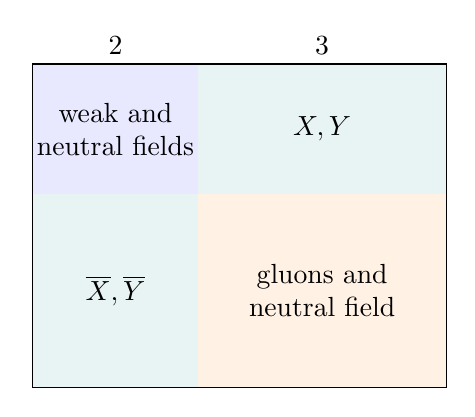
\begin{tikzpicture}[x=1.05cm,y=0.82cm]
  \draw[thick] (0,0) rectangle (5,5);
  \draw[thick] (2,0) -- (2,5);
  \draw[thick] (0,3) -- (5,3);
  \fill[blue!9] (0,3) rectangle (2,5);
  \fill[orange!10] (2,0) rectangle (5,3);
  \fill[teal!9] (2,3) rectangle (5,5);
  \fill[teal!9] (0,0) rectangle (2,3);
  \node[align=center] at (1,4) {weak and\\neutral fields};
  \node[align=center] at (3.5,1.5) {gluons and\\neutral field};
  \node[align=center] at (3.5,4) {\(X,Y\)};
  \node[align=center] at (1,1.5) {\(\overline X,\overline Y\)};
  \node[above] at (1,5) {\(2\)};
  \node[above] at (3.5,5) {\(3\)};
\end{tikzpicture}
\caption{The \(2\oplus3\) block structure of the \(SU(5)\) gauge field. The off-diagonal blocks connect leptons and colored fields.}
\label{fig:l10-gauge-blocks}
\end{figure}

With \(Q=T_3+Y\), the colored weak doublet in Eq.~\eqref{eq:l10-adjoint-sm} has charges \(-\tfrac13\) and \(-\tfrac43\); its conjugate has \(+\tfrac13\) and \(+\tfrac43\). The lecture calls these particles \(X\) and \(Y\) but explicitly declines to fix which name belongs to which charge. The transition and charge are the invariant content.

\begin{classroomqa}
\audiencequestion{Are there three versions of each new \(X\) or \(Y\) gauge boson? \lecturetimestamp{00:41:28}}
\lecturerresponse{Yes. A transition joins a colored quark entry to a colorless lepton entry, so the exchanged boson must carry the missing color. The \(X/Y\) fields form color triplets and can emit or absorb gluons.}
\end{classroomqa}

Colored particles are not observed as isolated asymptotic states. The new gauge bosons must decay or hadronize into color-neutral combinations, just as quarks do.

\section{Why the Multiplet Contains Anti-Down Quarks}

The generators of \(SU(N)\) are traceless Hermitian matrices. To see the connection with the word special, write an infinitesimal group element as
\begin{equation}
U(\epsilon)=e^{i\epsilon T}.
\end{equation}
Unitarity gives \(T^\dagger=T\), while
\begin{equation}
1=\det U=e^{i\epsilon\operatorname{tr}T}
\end{equation}
for arbitrary \(\epsilon\) gives
\begin{equation}
\operatorname{tr}T=0.
\label{eq:l10-traceless-generator}
\end{equation}

Electric charge is a linear combination of generators. On the matter column in Eq.~\eqref{eq:l10-fivebar}, it acts as
\begin{equation}
Q_{\overline5}
=
\operatorname{diag}
\left(0,-1,\frac13,\frac13,\frac13\right),
\qquad
\operatorname{tr}Q_{\overline5}=0.
\label{eq:l10-charge-fivebar}
\end{equation}
Thus
\begin{equation}
0-1+3\left(\frac13\right)=0.
\end{equation}
Replacing the anti-down fields by down fields would instead give
\begin{equation}
0-1+3\left(-\frac13\right)=-2,
\end{equation}
which cannot be the trace of an \(SU(5)\) generator. The apparently strange anti-down assignment is therefore forced by the group structure.

\section{The Remaining Ten Fermions}

The other ten fields arise from an antisymmetric two-index tensor. In the standard convention this is the antisymmetric part of
\begin{equation}
\mathbf5\otimes\mathbf5
=\mathbf{15}_S\oplus\mathbf{10}_A.
\label{eq:l10-five-five}
\end{equation}
The lecture constructs it by temporarily writing the conjugate quantum numbers
\begin{equation}
\chi=
\begin{pmatrix}
\nu^c\\
e^c\\
d_r\\
d_g\\
d_b
\end{pmatrix}.
\label{eq:l10-aux-five}
\end{equation}
This is a bookkeeping device for tensoring representations, not a claim that a second physical five-plet of composite particles exists.

Let
\begin{equation}
\Psi^{ij}=-\Psi^{ji},
\qquad
i,j=1,\ldots,5.
\label{eq:l10-antisym-ten}
\end{equation}
All diagonal entries vanish, and the lower triangle is fixed by the upper triangle. Hence
\begin{equation}
\dim\mathbf{10}
=\binom52
=\frac{5\cdot4}{2}
=10.
\label{eq:l10-ten-count}
\end{equation}

The electric charge of an entry is the sum of the row and column charges in Eq.~\eqref{eq:l10-aux-five}. This immediately gives \(e^c\) in the weak--weak slot, down and up quarks in the weak--color blocks, and anti-up fields in the color--color block.

\begin{classroomqa}
\audiencequestion{When the positron and down-quark labels are combined, should the resulting entry be an \(X\) boson? \lecturetimestamp{00:53:08}}
\lecturerresponse{No. At this stage we are constructing the fermion representation, not the gauge-boson adjoint. The charges add as \(1-\tfrac13=\tfrac23\), so the entry has the quantum numbers of an up quark.}
\end{classroomqa}

A consistent choice of color signs is
\begin{equation}
\Psi^{ij}=
\begin{pmatrix}
0 & e^c & d_r & d_g & d_b\\
-e^c & 0 & u_r & u_g & u_b\\
-d_r & -u_r & 0 & u_b^c & -u_g^c\\
-d_g & -u_g & -u_b^c & 0 & u_r^c\\
-d_b & -u_b & u_g^c & -u_r^c & 0
\end{pmatrix}.
\label{eq:l10-ten-matrix}
\end{equation}
Changing field phases changes some displayed signs but not the representation or particle content.

\begin{figure}[htbp]
\centering

\includegraphics[width=0.83\textwidth]{lecture_10_figure_05.png}
\lectureframe{00:59:17.500}
\caption{The unobstructed \(2\oplus3\) antisymmetric matter matrix after the entries and color labels have been checked in class.}
\label{fig:l10-ten-board}
\end{figure}

\begin{classroomqa}
\audiencequestion{Must the ten-dimensional representation be written as a matrix, or can it be written as a column? \lecturetimestamp{00:56:24}}
\lecturerresponse{Either is possible. One may list the ten independent components in a column, but the antisymmetric \(5\times5\) matrix displays how \(SU(5)\) acts on its two indices and is therefore much more informative.}
\end{classroomqa}

\begin{classroomqa}
\audiencequestion{In the color--color block, should the entry marked \(u\) actually be an anti-up field? \lecturetimestamp{00:57:51}}
\lecturerresponse{Yes. The board label is corrected to \(u^c\), a left-handed anti-up field. Two down-type basis charges sum to \(-\tfrac23\), which is the electric charge of an anti-up quark.}
\end{classroomqa}

\begin{classroomqa}
\audiencequestion{The colors were omitted from several matrix entries. Are they still conserved? \lecturetimestamp{00:58:05}}
\lecturerresponse{Yes. The three color slots are red, green, and blue. The labels were suppressed only to reduce clutter.}
\end{classroomqa}

An antisymmetric pair of color fundamentals transforms as an anti-color:
\begin{equation}
\wedge^2\mathbf3\simeq\overline{\mathbf3},
\qquad
(rg,rb,gb)\sim(\overline b,-\overline g,\overline r).
\label{eq:l10-anticolor}
\end{equation}
This is why the three independent entries in the color--color block form precisely the anti-up color triplet.

One generation has now been organized as
\begin{equation}
\overline{\mathbf5}\oplus\mathbf{10}.
\label{eq:l10-family}
\end{equation}
It is striking that \(u_L\) and \(u^c_L\) occur within one irreducible multiplet, while \(d_L\) and \(d^c_L\), or \(e_L\) and \(e^c_L\), lie in different multiplets.

\begin{classroomqa}
\audiencequestion{If gauge transformations act only within each representation, how can a mass connect fields lying in the five-bar and ten? \lecturetimestamp{01:00:40}}
\lecturerresponse{Gauge bosons do not rotate one irreducible matter representation into the other. Higgs fields and Yukawa couplings can connect different representations while forming an overall \(SU(5)\)-invariant interaction; after the Higgs field acquires an expectation value, those interactions generate masses.}
\end{classroomqa}

\section{Gauge Bosons Act as Shifts}

After the representation has been assembled, the action of a gauge boson can be read as a shift among its entries. A neutral boson may leave a label unchanged, a weak boson moves between weak slots, a gluon moves between color slots, and an \(X/Y\) boson moves between weak and color slots. Charged gauge bosons have antiparticles, so each shift has a reverse process.

For the antisymmetric tensor, an infinitesimal transformation acts on either index:
\begin{equation}
\delta\Psi^{ij}
=
i\epsilon
\left(
T^i{}_k\Psi^{kj}
+
T^j{}_k\Psi^{ik}
\right).
\label{eq:l10-two-index-action}
\end{equation}
In the matrix picture, the first term moves vertically and the second moves horizontally. The constituent labels used to build the tensor are only a mnemonic; Eq.~\eqref{eq:l10-two-index-action} is the exact group-theoretic statement.

Weak shifts take \(d\) into \(u\), the quark-level process behind neutron beta decay. Color shifts change red, green, and blue without changing flavor. Off-diagonal shifts do something new:
\begin{equation}
\begin{aligned}
d^c&\longleftrightarrow e,
& d^c&\longleftrightarrow\nu,\\
d&\longleftrightarrow u^c,
& u&\longleftrightarrow e^c,
\end{aligned}
\label{eq:l10-leptoquark-shifts}
\end{equation}
with the appropriate \(X/Y\) field carrying the charge and color difference.

\begin{classroomqa}
\audiencequestion{What do shifts between the fourth and fifth slots represent, and what about a shift from the first to the fourth? \lecturetimestamp{01:10:36}}
\lecturerresponse{The fourth--fifth shift changes one color into another and is a gluon transition. A first--fourth shift crosses between weak and color blocks and is one of the new \(X/Y\) transitions.}
\end{classroomqa}

\begin{classroomqa}
\audiencequestion{Can one entry of the lower half of the antisymmetric matrix be filled in explicitly? \lecturetimestamp{01:11:23}}
\lecturerresponse{Yes. Every lower-triangular entry is the negative of the transposed upper-triangular entry. Filling one makes the rule visible; filling all of them adds no new states.}
\end{classroomqa}

\section{The Dangerous Consequence: Proton Decay}

An \(X/Y\) boson can couple a quark to a lepton at one vertex and two quark-type fields at another. At momenta much smaller than its mass, integrating out the heavy boson gives a dimension-six interaction of the schematic form
\begin{equation}
\mathcal L_{\mathrm{eff}}
\sim
\frac{g_5^2}{M_X^2}\,(qq)(q\ell)
+\text{h.c.}
\label{eq:l10-effective-proton}
\end{equation}
It violates baryon and lepton number separately while preserving the combinations dictated by the unified gauge interaction.

The board follows one down quark and one up quark through the heavy exchange. The down quark becomes a positron, the up quark becomes an anti-up quark, and a second up quark is a spectator:
\begin{equation}
uud
\longrightarrow
e^++u\overline u.
\label{eq:l10-quark-decay}
\end{equation}
The initial state is a proton. The \(u\overline u\) pair can hadronize into a neutral pion, giving
\begin{equation}
p\longrightarrow e^++\pi^0.
\label{eq:l10-proton-pion}
\end{equation}

\begin{figure}[htbp]
\centering

\includegraphics[width=0.82\textwidth]{lecture_10_figure_06.png}
\lectureframe{01:16:02.500}
\caption{The completed board construction of the heavy-boson exchange inside a proton, with the spectator up quark and positron channel visible.}
\label{fig:l10-proton-board}
\end{figure}

The lecture also mentions \(p\to e^++\gamma\), in which the quark--antiquark pair annihilates electromagnetically. That channel carries an additional electromagnetic suppression relative to direct hadronization.

This possibility is not an optional decoration of the model. Once a simple group contains generators that connect quarks and leptons, baryon-number-violating processes are generally expected. If they occurred on ordinary weak or electromagnetic time scales, nuclei, hydrogen, and macroscopic matter would not survive.

\section{Why Is the Proton So Long-Lived?}

\begin{classroomqa}
\audiencequestion{Is the coupling that produces an \(X\) boson the same unified coupling used by the rest of the group? \lecturetimestamp{01:18:34}}
\lecturerresponse{At the unification scale, yes. A simple \(SU(5)\) gauge theory has one gauge coupling \(g_5\). The low-energy strong, weak, and hypercharge couplings differ because they run differently after the unified symmetry is broken.}
\end{classroomqa}

The coupling cannot be chosen fantastically small without abandoning the unified structure. The available suppression is the heavy propagator:
\begin{equation}
\mathcal A
\sim
\frac{g_5^2}{M_X^2}.
\label{eq:l10-amplitude}
\end{equation}
Squaring the amplitude supplies \(g_5^4/M_X^4\). Dimensional analysis and the proton matrix element complete the decay-rate estimate:
\begin{equation}
\Gamma_p
\sim
C_{\mathrm{had}}\,
\frac{\alpha_5^2\,m_p^5}{M_X^4},
\qquad
\alpha_5=\frac{g_5^2}{4\pi},
\label{eq:l10-rate}
\end{equation}
where \(C_{\mathrm{had}}\) contains group factors, renormalization effects, and the nonperturbative hadronic matrix element.

\editorialnote{The lecture isolates the essential \(g^4/M_X^4\) dependence and notes that proton-mass factors are omitted. Equation~\eqref{eq:l10-rate} restores the required mass dimension without claiming a precision lifetime calculation.}

\begin{classroomqa}
\audiencequestion{Does the small factor \(g^4\), perhaps of order \(10^{-8}\) in the rough classroom estimate, already make the lifetime long enough? \lecturetimestamp{01:25:13}}
\lecturerresponse{No. It helps, but the gap between a microscopic strong-interaction time and the proton-lifetime bound spans far more orders of magnitude. The fourth power of the heavy mass must provide the decisive suppression.}
\end{classroomqa}

If all masses were of order the proton mass, the natural time unit would be approximately the light-crossing time of a proton:
\begin{equation}
t_p\sim\frac{1\ \mathrm{fm}}{c}\sim10^{-23}\ \mathrm{s}.
\label{eq:l10-proton-time}
\end{equation}
The mere existence of primordial protons already shows that their lifetime exceeds the age of the universe, but laboratory searches go vastly further. The lecture compares the microscopic estimate with the then-quoted experimental limit
\begin{equation}
\tau_p\gtrsim10^{33}\ \mathrm{yr}.
\label{eq:l10-lifetime-bound}
\end{equation}

One need not watch a single proton for that long. If the lifetime were \(10^{15}\) years, a sample of \(10^{15}\) protons would yield roughly one event per year. More generally, with \(N_p\) protons observed for a time \(T\), the expected number of decays is
\begin{equation}
\langle n\rangle\simeq\frac{N_pT}{\tau_p}.
\label{eq:l10-event-count}
\end{equation}
A detector containing roughly \(10^{33}\) protons is a large tank rather than an astronomical object: the protons themselves have a mass of order \(10^6\) kilograms. Watching such a sample turns an enormous individual lifetime into a measurable event rate or a stronger lower bound.

Combining Eq.~\eqref{eq:l10-rate} with the lifetime constraint drives the leptoquark gauge-boson mass toward
\begin{equation}
M_X\sim10^{15}\text{--}10^{16}\ \mathrm{GeV},
\label{eq:l10-mx}
\end{equation}
with \(10^{16}\,\mathrm{GeV}\) used in the lecture as the memorable safe scale. This is several orders of magnitude below the Planck scale and therefore not automatically inconsistent with quantum field theory.

\section{Broken \texorpdfstring{\(SU(5)\)}{SU(5)} and the Unification Scale}

The \(X/Y\) fields share an \(SU(5)\) adjoint multiplet with the Standard Model gauge fields. Exact unbroken gauge symmetry would not permit some members to have masses near \(10^{16}\,\mathrm{GeV}\) while the photon and gluons remain massless. The symmetry must therefore be spontaneously broken.

\begin{classroomqa}
\audiencequestion{If the \(SU(5)\) symmetry were unbroken, would all of its gauge bosons be massless? \lecturetimestamp{01:29:37}}
\lecturerresponse{Yes, in the gauge theory under discussion. Gauge invariance forbids an explicit common mass. A Higgs mechanism can give masses to the gauge bosons associated with broken generators while leaving the unbroken subgroup gauge fields massless.}
\end{classroomqa}

The electroweak Higgs mechanism already illustrates the pattern: it distinguishes the photon from the \(W^\pm\) and \(Z\). Grand unification requires a separate high-scale order parameter that distinguishes the weak \(2\)-block from the color \(3\)-block and makes the off-diagonal \(X/Y\) fields extremely heavy.

Compared with \(10^{16}\,\mathrm{GeV}\), even a \(100\,\mathrm{GeV}\) weak-boson mass is negligible. Well above the heavy threshold, all gauge-boson masses may be neglected and the full \(SU(5)\) symmetry becomes a good approximation. This is the meaning of a unification scale: not that the low-energy world visibly has \(SU(5)\), but that sufficiently energetic processes become insensitive to the symmetry-breaking mass splittings.

\section{Running Couplings}

Gauge couplings depend logarithmically on the energy scale. Defining
\begin{equation}
\alpha_i(\mu)=\frac{g_i^2(\mu)}{4\pi},
\end{equation}
the one-loop evolution has the form
\begin{equation}
\alpha_i^{-1}(\mu)
=
\alpha_i^{-1}(\mu_0)
-\frac{b_i}{2\pi}
\ln\!\left(\frac{\mu}{\mu_0}\right).
\label{eq:l10-running}
\end{equation}
The coefficients \(b_i\) depend on the gauge group and on every particle light enough to circulate in the relevant quantum loops.

\editorialnote{To compare hypercharge with the non-Abelian couplings inside \(SU(5)\), \(g_1\) must be given the conventional grand-unified normalization. This is the source of the numerical group-theory factors mentioned in the lecture.}

At laboratory energies, the inverses of the three couplings are different. In the lecture's qualitative ordering, \(1/\alpha_1\) is largest because hypercharge is weakest, \(1/\alpha_2\) comes next, and \(1/\alpha_3\) is smallest because the strong interaction is strongest. The curves at inaccessible energies are not directly measured. They are calculated from the observed low-energy values, the particle spectrum, and the loop diagrams that determine the beta functions. With the Standard Model particle content they become nearly straight lines when plotted against \(\log\mu\).

\begin{figure}[htbp]
\centering

\includegraphics[width=0.74\textwidth]{lecture_10_figure_07.png}
\lectureframe{01:36:32.500}
\caption{The board plot of the inverse gauge couplings approaching one another near \(10^{16}\,\mathrm{GeV}\). The circled region marks their imperfect meeting.}
\label{fig:l10-running-board}
\end{figure}

Below the unification threshold the symmetry is broken, the light spectrum does not fill complete degenerate \(SU(5)\) multiplets, and the three beta-function coefficients differ. Consequently the couplings run at different rates. At the high scale one asks whether they reach a common value:
\begin{equation}
\alpha_1(M_{\mathrm{GUT}})
\stackrel{?}{=}
\alpha_2(M_{\mathrm{GUT}})
\stackrel{?}{=}
\alpha_3(M_{\mathrm{GUT}}).
\label{eq:l10-unification-condition}
\end{equation}

With only the nonsupersymmetric Standard Model spectrum, the lines approach one another around \(10^{15}\)--\(10^{16}\,\mathrm{GeV}\) but miss by an appreciable amount; the lecture describes the agreement as roughly fifteen percent. The important coincidence is that this is also the scale demanded by proton stability.

\section{A Final Neutron Question}

\begin{classroomqa}
\audiencequestion{If the spectator up quark in the proton-decay diagram were replaced by a down quark, would this describe neutron decay, and would the \(X\) boson matter? \lecturetimestamp{01:36:40}}
\lecturerresponse{It would define a grand-unified neutron channel such as \(n\to e^++\pi^-\), but that is not the familiar decay of a free neutron. Ordinary neutron beta decay is \(n\to p+e^-+\overline\nu_e\) and proceeds through the weak interaction. If the proton--neutron mass ordering were reversed, beta stability would be reversed as well, while the much slower grand-unified channel could remain.}
\end{classroomqa}

This distinction separates kinematics from the new interaction. Which nucleon beta-decays depends on the proton--neutron mass difference; baryon-number violation from \(X/Y\) exchange is a separate, enormously suppressed mechanism.

\section{Supersymmetry and the Larger Perspective}

Adding a supersymmetric partner spectrum changes the beta-function coefficients in Eq.~\eqref{eq:l10-running}. In the lecture's account, the three extrapolated couplings then meet to about one-percent accuracy. This does not prove supersymmetry or grand unification, but it is the empirical reason the two ideas are often discussed together.

The matter multiplets can be unified still further. Under
\begin{equation}
SO(10)\supset SU(5),
\end{equation}
one spinor representation decomposes as
\begin{equation}
\mathbf{16}
\longrightarrow
\mathbf{10}\oplus\overline{\mathbf5}\oplus\mathbf1.
\label{eq:l10-so10}
\end{equation}
The singlet is naturally identified with a left-handed antineutrino, or equivalently the charge conjugate of a right-handed neutrino. Thus all sixteen fields of an extended family fit into one irreducible \(SO(10)\) multiplet.

Proton-decay experiments continue to test the idea by raising the lifetime bound when no event is seen. Supersymmetric grand-unified models do not give one universal proton lifetime: additional heavy fields and superpartner-dependent operators can change the dominant channel and rate over a broad range.

\editorialnote{In supersymmetric grand unification, color-triplet Higgs exchange can generate dimension-five baryon-violating operators in addition to the dimension-six gauge-boson operator discussed here. Their coefficients depend strongly on the heavy spectrum, flavor structure, and superpartner masses, which explains the lecture's warning that no single lifetime follows from supersymmetry alone.}

The lasting lesson is a tension rather than a verdict. The group theory fits quarks and leptons together with remarkable economy, the running couplings hint at a common high scale, and supersymmetry sharpens the numerical hint. The same construction also predicts the dangerous conversion of quarks into leptons. Any successful version must therefore preserve the elegance while keeping the proton stable for an almost inconceivably long time. In the lecture's closing spirit: may all our protons remain stable.
